% Document uses 12 pt font
% 1 in margins
% Contains a relative path for images

\documentclass [10pt]{article}
\usepackage{float}

% page geometry 
\usepackage[margin=1in]{geometry}


% ----------  PACKAGES START ------------ %
% Math Packages
\usepackage{amsmath}
\usepackage{mathtools}

% Table cell color package and highlighting
\usepackage[table]{xcolor}
\usepackage{color,soul}

% VIC title package
\usepackage{cabin}
\usepackage[T1]{fontenc}

% default font package
%\usepackage{times}
\usepackage{helvet}
%\renewcommand{\familydefault}{\sfdefault}

% ---------- End Font Packages -------------- %

\usepackage{listings}


\definecolor{dkgreen}{rgb}{0,0.6,0}
\definecolor{gray}{rgb}{0.5,0.5,0.5}
\definecolor{mauve}{rgb}{0.58,0,0.82}

\lstset{frame=tb,
  language=C++,
  aboveskip=3mm,
  belowskip=3mm,
  showstringspaces=false,
  columns=flexible,
  basicstyle={\small\ttfamily},
  numbers=none,
  numberstyle=\tiny\color{gray},
  keywordstyle=\color{blue},
  commentstyle=\color{dkgreen},
  stringstyle=\color{mauve},
  breaklines=true,
  breakatwhitespace=true,
  tabsize=3
}

% Title Packages
\usepackage{titlesec}
\usepackage{titletoc}

% Image Package
\usepackage{graphicx}

% Table Packages
\usepackage{longtable}
\usepackage{multirow}
\usepackage{multicol}
\usepackage{multirow}
\usepackage{array}
\renewcommand{\arraystretch}{1.2}% Spread rows out evenly in table
\setlength{\LTpre}{0.5pt} % Reduces white space around tables (top)
%\setlength{\LTpost}{0pt} % Reduces white space around tables (bottom)

% Color Packages
\usepackage{color}   
\definecolor{sectionC}{rgb}{0.95,0.52,.0}
\definecolor{subsectionC}{rgb}{1.0,.64,.26}
\definecolor{subsubsectionC}{rgb}{1.0,.87,.68}
\definecolor{tableCell}{rgb}{.98,.81,.69}


% List package
\usepackage{enumitem}
\setenumerate{itemsep=0pt, itemindent=0in,leftmargin=0.5in}


% Paragraph parameter
\usepackage{lscape}
\setlength{\parindent}{0pt}


% ------------- Creates a linked Table of Contents  Start --------------- %
\usepackage{hyperref}
\hypersetup{
colorlinks=true, %set true if you want colored links
linktoc=all,     %set to all if you want both sections and subsections linked
linkcolor=black,}  %choose some color if you want links to stand out

% ------------- Creates a click-able Table of Contents  End--------------- %

% ---------- PACKAGES END ------------ %








% -------- SECTION AND SUBSECTION FORMATING START -------- % 
% starts the 
%\setcounter{section}{1}


\titleformat{\section} % Section
{\normalfont \fontsize{14}{14} \bfseries}{}{0em}{\colorsection}

% Makes a background color
\newcommand{\colorsection}[1]{%
  \colorbox{sectionC}{\parbox{\dimexpr\textwidth-1\fboxsep}{\color{white}\Large\thesection\ \hspace{1mm} #1}}}

% Makes a background color
\titleformat{\subsection} % Subsection
{\normalfont \fontsize{12}{12}  \bfseries}{}{0em}{\colorsubsection }

\newcommand{\colorsubsection}[1]{%
  \colorbox{subsectionC}{\parbox{\dimexpr \textwidth -1\fboxsep}{\large\thesubsection\ #1}}}


% Makes a background color
\titleformat{\subsubsection} % Subsubsection
{\normalfont \fontsize{12}{12} \bfseries}{}{0em}{\colorsubsubsection}

\newcommand{\colorsubsubsection}[1]{%
  \colorbox{subsubsectionC}{\parbox{\dimexpr\textwidth-1\fboxsep}{\thesubsubsection\ #1}}}

% -------- SECTION AND SUBSECTION FORMATING END -------- % 
\usepackage{lipsum}


% -----  IMAGE PATH START -----%
% Relative Image Path
\graphicspath {figures/}
% -----  IMAGE PATH END -----%

% ------ PARAGRAPH FORMAT START ----%
%\setlength{\parskip}{.2em}% Sets the space between new paragraph items 
\setlength{\parindent}{0em} % paragraph indent
% ------ PARAGRAPH FORMAT END ----%




%------------------------------TOC FORMAT START --------------------------------%
\usepackage{tocloft}



% Section indentations
\cftsetindents{section}{0em}{1.5em}
\cftsetindents{subsection}{1em}{2em}
\cftsetindents{subsubsection}{2em}{3em}

% Toc title size
\renewcommand\cfttoctitlefont{\Large\bfseries}
\renewcommand*\contentsname{Table of Contents}

\newcommand{\carSpeed}{1.4\ m/s}
\newcommand{\intersectionLength}{0.6\ m}


% Removes bold headings from toc
%\renewcommand{\cftsecfont}{\normalfont}

% Removes bold heading page numbers from toc
\renewcommand{\cftsecpagefont}{\normalfont}

% add dots after headings
%\renewcommand{\cftsecleader}{\cftdotfill{\cftdotsep}} 


% number of section headings we want to see in toc
\setcounter{tocdepth}{2}

% Spaceing before headings in toc
\setlength{\cftbeforesecskip}{6pt}

% ------------------------------TOC FORMAT END --------------------------------%



% ------------------- START HEADER AND FOOTER ---------------------------%
\usepackage{fancyhdr}

% Helps with the n of total n pages
\usepackage{lastpage}

\pagestyle{fancy}

% Header
\lhead{Draft Hazard Analysis}
\rhead{Revision: 1}
\fancyhead[LE,CO]{Group 9: LazyBots}

% Removes line under the header 
\renewcommand{\headrulewidth}{0pt}
\setlength{\headsep}{.2in}

% Footer 

% Set the right side of the footer to be the page number
\fancyfoot[R]{Page \textbf{\thepage}\ of \textbf{\pageref{LastPage}}}
\fancyfoot[C]{}

% ------------------- END HEADER AND FOOTER ---------------------------%






% -------------- DOCUMENT START ---------------%
\begin{document}

% --------- TITLE PAGE START ------- %
\begin {center} 

\thispagestyle{empty}
\vspace*{5cm}

% Logo Insertion
\begin {figure}[h!]
\centering
\hspace{-10mm}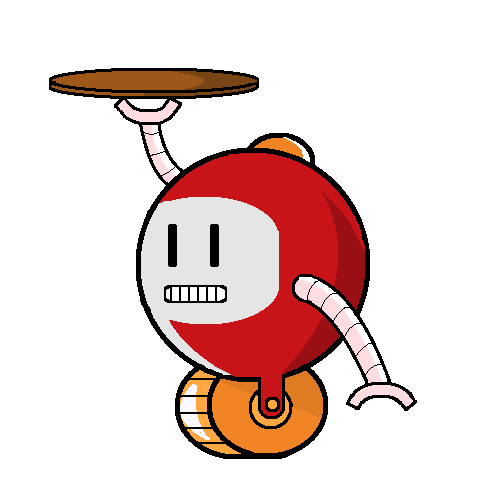
\includegraphics [scale = .3, trim={.4cm 0 .8cm 0},clip] {figures/alfred.png}
\end {figure}

{\fontfamily{\cabinfamily}\selectfont
\Huge{LazyBots} }

\vspace{1 cm}
{\Large\textbf{\textsc{McMaster University}}\\}  \vspace {1cm}
{\Large Hazard Analysis\\ \vspace {0.4 cm} SE 4GA6 \& TRON 4TB6}  \vspace {1cm}

{\large \textsc{Group 9} \\} \vspace{1cm}



\begin{tabular}{ l c  l}
Karim Guirguis & & 001307668 \\
David Hemms & & 001309228 \\
Marko Laban & & 001300989 \\
Curtis Milo & & 001305877 \\
Keyur Patel & & 001311559 \\
Alexandra Rahman & & 001305735
\end{tabular}


\end{center}


% --------- TITLE PAGE END------- %

\pagebreak

% Inserting table of contents and table of figures 

\tableofcontents
\listoftables
\listoffigures



\pagebreak

% -----------  REVISION HISTORY START ----------- %

%\section*{Revisions}
\thispagestyle{empty}
\section{Revisions}
\begin{longtable}{| p{.2\textwidth } | p{.23\textwidth } | p{.23\textwidth } | p{.23\textwidth } |} 

% ------------------------------------------------------- Date ------------------------------------------------------- %
\hline 
\centering \textbf{Date} & 
\multicolumn{1}{c}{\textbf {Revision Number}} &
\multicolumn{1}{|c}{\textbf {Authors}} & 
\multicolumn{1}{|c|}{\textbf {Comments}} \\ \hline

% ------------------------------------------------------- Revision Number -------------------------------------------------------
\multirow{4}{*}{\centering November 24\textsuperscript{th}, 2017}  & 
\multirow{4}{*}{Revision 0}& 
		{Karim Guirguis \newline
		David Hemms \newline
		Marko Laban \newline
		Curtis Milo \newline
		Keyur Patel \newline
		Alexandra Rahman} &
 \multirow{4}{*}{-} \\ 
\hline 

\multirow{4}{*}{\centering March 6\textsuperscript{th}, 2018}  & 
\multirow{4}{*}{Revision 1}& 
		{Karim Guirguis \newline
		David Hemms \newline
		Marko Laban \newline
		Curtis Milo \newline
		Keyur Patel \newline
		Alexandra Rahman} &
{Added the section to include the scope of the project as well as edited the FMEA table to include hazards that have been previously overlooked. }\\
\hline 

\caption{LazyBots Table of Revisions}
\end{longtable}



\pagebreak

%---------------------------- PROJECT DRIVERS ------------------------%
% heading in document

% ------------------------------------------------------- INTRODUCTION ------------------------------------------------------- %

\section {Introduction}

% ------------------------------------------------------- Document Purpose ------------------------------------------------------- %
\subsection{Document Purpose}
The purpose of this document is to identify the components of Alfred which could potentially have hazardous consequences, and either eliminate them or reduce its risk to an acceptable level. Hazard analysis should be performed for all the major phases of the software development lifecycle, including requirements, architectural design, detailed design, and actual code. In particular, this document will look at the hazardous potential when the system works correctly, as well as when the system works incorrectly. \\ \newline
Hazards will be identified based on hazards from similar systems, as well as any hazards that occur during development/lifecycle of the system.\\ \newline
For this report we will analyze the hazards which can be affected by our mechanical and software systems.

% --------------------------------------------------------------- Scope --------------------------------------------------------------- %
\subsection{Scope}
The system implemented is one that is meant to automate the dispensing of beverages to customers within a restaurant at the respective customers' table. The customer will be able to order a drink from their table which will be followed by Alfred arriving at their table and dispensing the requested drinks. The staff will be able to request Alfred to return to a Home Base for charging and refilling when desired. 

% ------------------------------------------------------------ Definitions ------------------------------------------------------------ %
\subsection{Definitions}

\begin{longtable}{| p{.25\textwidth} | p{.70\textwidth} |}\hline
	\rowcolor{tableCell}\textbf{System Hazard} & The system is in a condition/state from which an accident can occur.\\ \hline
	\textbf{Accident} & Unplanned event which can lead to unacceptable consequences. \\ \hline
	\rowcolor{tableCell}\textbf{Risk} & A measure that combines the likelihood that a system hazard will happen, the likelihood that an accident will happen, and the severity of the worst potential accident.\\ \hline
	\textbf{Critical System} & System whose failure can lead to unacceptable consequences.\\ \hline
	\rowcolor{tableCell}\textbf{Safety Critical System} & A critical system whose failure can lead to injury, death, or environmental damage.\\ \hline
\end{longtable}


% ---------------------------------------------------- COMPONENT OVERVIEW --------------------------------------------------- %
\section{Component Overview}
The components can be divided into the following ten components:

% ------------------------------------------------------ Drink Ordering System ------------------------------------------------------- %
\subsection{Drink Ordering System}
An android application that allows customers and consumers to order drinks. The order is then relayed to Alfred.

% ------------------------------------------------------ Login System ------------------------------------------------------- %
\subsection{Login System}
A web application that allows users such as administrators or servers to login into the system and modify the restaurant map or close orders.

% --------------------------------------------------- Administrative Map System ---------------------------------------------------- %
\subsection{Administrative Map System}
An android application that allows an administrator to change the layout of the restaurant. This map is then relayed to Alfred.

% --------------------------------------------------- Error Management System ---------------------------------------------------- %
\subsection{Error Management System}
An application that allows users and administrators to view and track ongoing issues with Alfred. Users can also close issues once they have been resolved. 

% --------------------------------------------------- Backend Server System ---------------------------------------------------- %
\subsection{Backend Server System}
The backend server serves as a method of communication between Alfred and other applications and components.

% --------------------------------------------------- Alfred Manager System ---------------------------------------------------- %
\subsection{Alfred Manager System}
This system serves as Alfred's drink order manager. The system will place the orders in a queue and assign them to the corresponding table number so that Alfred may complete the drink order.

% --------------------------------------------------- Drivetrain Subsystem ---------------------------------------------------- %
\subsection{Drivetrain Subsystem}
This is the basic mechanical and electrical components of Alfred that allow motion and movement. 

% --------------------------------------------------- Alfred Pumping System ---------------------------------------------------- %
\subsection{Alfred Pumping System}
The system that deals with the fluid dynamics. Receives necessary information from Alfred Manager System to dispense correct type of drink, with the correct amount for the corresponding table. 

% ------------------------------------------------- Image Processing  Subsystem -------------------------------------------------- %
\subsection{Image Processing Subsystem}
Alfred will be utilizing this subsystem to assure that all pathways are clear and to relay better error reports in case on an accident.




% -------------------------------------------------- SAFETY CONSIDERATIONS -------------------------------------------------- %
\section{Safety Considerations}

% ------------------------------------------------------ Drink Ordering System ------------------------------------------------------- %
\subsection{Drink Ordering System}
	\textbf{Software Issues:}
		\begin {itemize}
			\item An order is not sent within the desired time
		\end {itemize}
		
	\textbf{Hardware Issues:}
		\begin {itemize}
			\item None
		\end {itemize}

% ------------------------------------------------------ Login System ------------------------------------------------------- %
\subsection{Login System}
	\textbf{Software Issues:}
		\begin {itemize}
			\item The ability to perform attacks the server software to prevent access to the system
			\item The ability to perform attacks the server software to pose as store manager
			\item The ability to snoop information in order to obtain information about clients
			\item The ability to attack the system by injecting code
		\end {itemize}
		
	\textbf{Hardware Issues:}
		\begin {itemize}
			\item Server is not able to perform functionality to properly verify users due to internet issues or component failure
		\end {itemize}
% --------------------------------------------------- Administrative Map System ---------------------------------------------------- %
\subsection{Administrative Map System}
	\textbf{Software Issues:}
		\begin {itemize}
			\item The ability to inject false information while data is being transferred to the server 
		\end {itemize}
		
	\textbf{Hardware Issues:}
		\begin {itemize}
			\item Computer is not able to perform functionality due to internet issues or component failure
		\end {itemize}
% --------------------------------------------------- Error Management System ---------------------------------------------------- %
\subsection{Error Management System}
	\textbf{Software Issues:}
		\begin {itemize}
			\item Errors are injected into the communication to be able to provide incorrect information to the manager's system
			\item Errors are not received within the desired time
		\end {itemize}
		
	\textbf{Hardware Issues:}
		\begin {itemize}
			\item Computer is not able to perform functionality due to internet issues or component failure
		\end {itemize}
% --------------------------------------------------- Backend Server System ---------------------------------------------------- %
\subsection{Backend Server System}
	\textbf{Software Issues:}
		\begin {itemize}
			\item The ability to perform attacks the server to prevent access to the system
			\item The ability to perform attacks the server system to pose as a manager or administrator
			\item The ability to snoop information in order to obtain information about clients
			\item The ability to attack the system by injecting code
			\item Issues with response and processing time of the subsystem
		\end {itemize}
		
	\textbf{Hardware Issues:}
		\begin {itemize}
			\item Server is not able to perform functionality to properly verify users due to internet issues or component failure
		\end {itemize}
% --------------------------------------------------- Alfred Manager System ---------------------------------------------------- %
\subsection{Alfred Manager System}
	\textbf{Software Issues:}
		\begin {itemize}
			\item Attacks where incorrect drink orders are sent to Alfred
		\end {itemize}
		
	\textbf{Hardware Issues:}
		\begin {itemize}
			\item Issues within micro-controller that would prevent computation functionality
			\item Issues such as faulty wiring or noise would prevent proper communication to the drink subsystem
		\end {itemize}
% --------------------------------------------------- Drivetrain Subsystem ---------------------------------------------------- %
\subsection{Drivetrain Subsystem}
	\textbf{Software Issues:}
		\begin {itemize}
			\item Correct command to the motor is obtained and is regulated for things such as slew rates and max capacities
			\item The system is within a stable control state of operation and if not the ensuring that there is no motion
			\item Detection of obstacles blocking Alfred's path of motion
		\end {itemize}
		
	\textbf{Hardware Issues:}
		\begin {itemize}
			\item Encoders are operating within the normal suggested operating range
			\item Motors are performing the correct path of motion based on the control systems specifications
			\item Motors are performing within the recommended operating range
			\item Ultrasonic sensors are providing information within the recommended operating range
			\item Electrical components being leaked on by liquid storage devices
			\item Insufficient power is supplied from the battery to the drive system
		\end {itemize}
% --------------------------------------------------- Alfred Pumping System ---------------------------------------------------- %
\subsection{Alfred Pumping System}
	\textbf{Software Issues:}
		\begin {itemize}
			\item The software system is not able to validate command from the Alfred manager system
		\end {itemize}
		
	\textbf{Hardware Issues:}
		\begin {itemize}
			\item There is a leak within the pumping system
			\item There is a leak within the storage of the liquids
			\item Alfred is not able to pump liquid using the pump
			\item Micro-controller is not able to receive information due to broken communication lines
			\item Micro-controller components fail and is not able to process drink request
		\end {itemize}
% ------------------------------------------------- Image Processing  Subsystem -------------------------------------------------- %
\subsection{Image Processing Subsystem}
	\textbf{Software Issues:}
		\begin {itemize}
			\item The software image processing Library is not able to properly process the image due to poor lighting conditions
		\end {itemize}
		
	\textbf{Hardware Issues:}
		\begin {itemize}
			\item The image is not able to be captured properly due to a broken or blocked camera
			\item Micro-controller processor is broken and not able to perform functionality
		\end {itemize}


\pagebreak 



% --------------------------------------- Relation between Hazards and Requirements -------------------------------------- %
\section{Correlation Between Hazard Functions and  Requirements}

% --------------------------------------- Hazard Function 1 -------------------------------------- %

\begin{table}[H]
\centering
\begin{tabular}{|c|l|lll}
\cline{1-2}
\textbf{Hazard Function:} & \multicolumn{1}{c|}{\textbf{Functional and Non-Functional Requirement:}} &  &  &  \\ \cline{1-2}
\multirow{9}{*}{F1: Movement of Alfred} 
				& Alfred Functional Requirement 3		&  &  &  \\ \cline{2-2}
                                  & Alfred Functional Requirement 10		&  &  &  \\ \cline{2-2}
                                  & Alfred Functional Requirement 11		&  &  &  \\ \cline{2-2}
                                  & Alfred Functional Requirement 12		&  &  &  \\ \cline{2-2}
                                  & Non-Functional Requirement 11		&  &  &  \\ \cline{2-2}
                                  & Non-Functional Requirement 13 		&  &  &  \\ \cline{2-2}
                                  & Non-Functional Requirement 16 		&  &  &  \\ \cline{2-2}
                                  & Non-Functional Requirement 18		&  &  &  \\ \cline{2-2}
                                  & Non-Functional Requirement 20		&  &  &  \\ \cline{1-2}
\end{tabular}
\caption{Correlation between Hazard Function 1 and Requirements}  
\end{table}


% --------------------------------------- Hazard Function 2 -------------------------------------- %

\begin{table}[H]
\centering
\begin{tabular}{|c|l|lll}
\cline{1-2}
\textbf{Hazard Function:}  & \multicolumn{1}{c|}{\textbf{Functional and Non-Functional Requirement:}} &  &  &  \\ \cline{1-2}
\multirow{8}{*}{F2: Correlates drink order to correct table} 
					& Alfred Functional Requirement 1			&  &  &  \\ \cline{2-2}
                                          & Alfred Functional Requirement 2			&  &  &  \\ \cline{2-2}
                                          & Alfred Functional Requirement 4			&  &  &  \\ \cline{2-2}
                                          & Alfred Functional Requirement 8			&  &  &  \\ \cline{2-2}
                                          & Alfred Functional Requirement 14			&  &  &  \\ \cline{2-2}
                                          & Table Ordering Functional Requirement 2	&  &  &  \\ \cline{2-2}
                                          & Non-Functional Requirement 14			&  &  &  \\ \cline{2-2}
                                          & Non-Functional Requirement 15 			&  &  &  \\ \cline{1-2}
\end{tabular}
\caption{Correlation between Hazard Function 2 and Requirements}  
\end{table}


% --------------------------------------- Hazard Function 3 -------------------------------------- %


\begin{table}[H]
\centering
\begin{tabular}{|c|l|lll}
\cline{1-2}
\textbf{Hazard Function:} & \multicolumn{1}{c|}{\textbf{Functional and Non-Functional Requirement:}} &  &  &  \\ \cline{1-2}
\multirow{5}{*}{F3: Navigates to table successfully} 
				& Alfred Functional Requirement 3		&  &  &  \\ \cline{2-2}
                                  & Alfred Functional Requirement 10		&  &  &  \\ \cline{2-2}
                                  & Non-Functional Requirement 11		&  &  &  \\ \cline{2-2}
                                  & Non-Functional Requirement 13 		&  &  &  \\ \cline{2-2}
                                  & Non-Functional Requirement 16 		&  &  &  \\ \cline{2-2}
                                  & Non-Functional Requirement 20		&  &  &  \\ \cline{1-2}
\end{tabular}
\caption{Correlation between Hazard Function 1 and Requirements}  
\end{table}


% --------------------------------------- Hazard Function 4 -------------------------------------- %


\begin{table}
\centering
\begin{tabular}{|c|l|lll}
\cline{1-2}
\textbf{Hazard Function:} & \multicolumn{1}{c|}{\textbf{Functional and Non-Functional Requirement:}} &  &  &  \\ \cline{1-2}
\multirow{13}{*}{F4: Dispense correct drink for the order} 
				& Alfred Functional Requirement 1	&  &  &  \\ \cline{2-2}
                                  & Alfred Functional Requirement 2	&  &  &  \\ \cline{2-2}
                                  & Alfred Functional Requirement 4 	&  &  &  \\ \cline{2-2}
                                  & Alfred Functional Requirement 6	&  &  &  \\ \cline{2-2}
                                  & Alfred Functional Requirement 7	&  &  &  \\ \cline{2-2}
				& Alfred Functional Requirement 8	&  &  &  \\ \cline{2-2}
				& Alfred Functional Requirement 9	&  &  &  \\ \cline{2-2}
                                  & Non-Functional Requirement 14	&  &  &  \\ \cline{2-2}
                                  & Non-Functional Requirement 17	&  &  &  \\ \cline{2-2}
                                  & Non-Functional Requirement 21	&  &  &  \\ \cline{2-2}
                                  & Non-Functional Requirement 26	&  &  &  \\ \cline{2-2}
                                  & Non-Functional Requirement 31	&  &  &  \\ \cline{2-2}
                                  & Non-Functional Requirement 33	&  &  &  \\ \cline{1-2}
\end{tabular}
\caption{Correlation between Hazard Function 4 and Requirements}  
\end{table}


% --------------------------------------- Hazard Function 5 -------------------------------------- %


\begin{table}
\centering
\begin{tabular}{|c|l|lll}
\cline{1-2}
\textbf{Hazard Function:} & \multicolumn{1}{c|}{\textbf{Functional and Non-Functional Requirement:}} &  &  &  \\ \cline{1-2}
\multirow{7}{*}{F5: Dispense correct amount} 
				& Alfred Functional Requirement 1	&  &  &  \\ \cline{2-2}
                                  & Alfred Functional Requirement 2	&  &  &  \\ \cline{2-2}
                                  & Alfred Functional Requirement 4	&  &  &  \\ \cline{2-2}
                                  & Alfred Functional Requirement 5	&  &  &  \\ \cline{2-2}
                                  & Alfred Functional Requirement 8	&  &  &  \\ \cline{2-2}
                                  & Alfred Functional Requirement 9	&  &  &  \\ \cline{2-2}
                                  & Non-Functional Requirement 12	&  &  &  \\ \cline{2-2}
                                  & Non-Functional Requirement 19	&  &  &  \\ \cline{2-2}
                                  & Non-Functional Requirement 21	&  &  &  \\ \cline{1-2}
\end{tabular}
\caption{Correlation between Hazard Function 5 and Requirements}  
\end{table}


% --------------------------------------- Hazard Function 6 -------------------------------------- %


\begin{table}
\centering
\begin{tabular}{|c|l|lll}
\cline{1-2}
\textbf{Hazard Function:} & \multicolumn{1}{c|}{\textbf{Functional and Non-Functional Requirement:}} &  &  &  \\ \cline{1-2}
\multirow{7}{*}{F6: Determine when liquids are not the correct temperature} 
				      & Alfred Functional Requirement 6	&  &  &  \\ \cline{2-2}
                                        & Alfred Functional Requirement 7	&  &  &  \\ \cline{2-2}
                                        & Administration Functional Requirement 5	&  &  &  \\ \cline{2-2}
                                        & Non-Functional Requirement 17	&  &  &  \\ \cline{2-2}
                                        & Non-Functional Requirement 25	&  &  &  \\ \cline{2-2}
                                        & Non-Functional Requirement 34	&  &  &  \\ \cline{2-2}
                                        & Non-Functional Requirement 35	&  &  &  \\ \cline{1-2}
\end{tabular}
\caption{Correlation between Hazard Function 6 and Requirements}  
\end{table}


% --------------------------------------- Hazard Function 7 -------------------------------------- %

\begin{table}
\centering
\begin{tabular}{|c|l|lll}
\cline{1-2}
\textbf{Hazard Function:} & \multicolumn{1}{c|}{\textbf{Functional and Non-Functional Requirement:}} &  &  &  \\ \cline{1-2}
\multirow{8}{*}{F7: Notify staff when errors or warnings occur} 
				      & Alfred Functional Requirement 6	&  &  &  \\ \cline{2-2}
                                        & Alfred Functional Requirement 7	&  &  &  \\ \cline{2-2}
                                        & Alfred Functional Requirement 8	&  &  &  \\ \cline{2-2}
                                        & Alfred Functional Requirement 10	&  &  &  \\ \cline{2-2}
                                        & Alfred Functional Requirement 11	&  &  &  \\ \cline{2-2}
                                        & Administration Functional Requirement 4	&  &  &  \\ \cline{2-2}
                                        & Non-Functional Requirement 26	&  &  &  \\ \cline{2-2}
                                        & Non-Functional Requirement 27	&  &  &  \\ \cline{2-2}
                                        & Non-Functional Requirement 31	&  &  &  \\ \cline{2-2}
                                        & Non-Functional Requirement 33	&  &  &  \\ \cline{1-2}
\end{tabular}
\caption{Correlation between Hazard Function 7 and Requirements}  
\end{table}


% --------------------------------------- Hazard Function 8 -------------------------------------- %


\begin{table}
\centering
\begin{tabular}{|c|l|lll}
\cline{1-2}
\textbf{Hazard Function:} & \multicolumn{1}{c|}{\textbf{Functional and Non-Functional Requirement:}} &  &  &  \\ \cline{1-2}
\multirow{3}{*}{F8: Determine when liquid supply is lower than desired level} 
				      & Alfred Functional Requirement 7	&  &  &  \\ \cline{2-2}
                                        & Alfred Functional Requirement 8	&  &  &  \\ \cline{2-2}
                                        & Alfred Functional Requirement 9	&  &  &  \\ \cline{2-2}
                                        & Administration Functional Requirement 5	&  &  &  \\ \cline{2-2}
                                        & Non-Functional Requirement 22	&  &  &  \\ \cline{1-2}
\end{tabular}
\caption{Correlation between Hazard Function 8 and Requirements}  
\end{table}


% --------------------------------------- Hazard Function 9 -------------------------------------- %


\begin{table}
\centering
\begin{tabular}{|c|l|lll}
\cline{1-2}
\textbf{Hazard Function:} & \multicolumn{1}{c|}{\textbf{Functional and Non-Functional Requirement:}} &  &  &  \\ \cline{1-2}
\multirow{4}{*}{F9: Moving the liquid storage containers} 
				      & Alfred Functional Requirement 10	&  &  &  \\ \cline{2-2}
                                        & Non Functional Requirement 1		&  &  &  \\ \cline{2-2}
                                        & Non Functional Requirement 1	3	&  &  &  \\ \cline{2-2}
                                        & Non Functional Requirement 1	8	&  &  &  \\ \cline{2-2}
                                        & Non-Functional Requirement 22	&  &  &  \\ \cline{1-2}
\end{tabular}
\caption{Correlation between Hazard Function 9 and Requirements}  
\end{table}


% --------------------------------------- Hazard Function 10 -------------------------------------- %


\begin{table}
\centering
\begin{tabular}{|c|l|lll}
\cline{1-2}
\textbf{Hazard Function:} & \multicolumn{1}{c|}{\textbf{Functional and Non-Functional Requirement:}} &  &  &  \\ \cline{1-2}
\multirow{18}{*}{F10: Dispense drink for the customer} 
				& Alfred Functional Requirement 1	&  &  &  \\ \cline{2-2}
                                  & Alfred Functional Requirement 2	&  &  &  \\ \cline{2-2}
                                  & Alfred Functional Requirement 3	&  &  &  \\ \cline{2-2}
                                  & Alfred Functional Requirement 4 	&  &  &  \\ \cline{2-2}
                                  & Alfred Functional Requirement 6	&  &  &  \\ \cline{2-2}
				& Alfred Functional Requirement 8	&  &  &  \\ \cline{2-2}
				& Alfred Functional Requirement 9	&  &  &  \\ \cline{2-2}
				& Alfred Functional Requirement 10	&  &  &  \\ \cline{2-2}
				& Table Ordering Functional Requirement 2	&  &  &  \\ \cline{2-2}
                                  & Non-Functional Requirement 11	&  &  &  \\ \cline{2-2}
                                  & Non-Functional Requirement 12	&  &  &  \\ \cline{2-2}
                                  & Non-Functional Requirement 13	&  &  &  \\ \cline{2-2}
                                  & Non-Functional Requirement 14	&  &  &  \\ \cline{2-2}
                                  & Non-Functional Requirement 16	&  &  &  \\ \cline{2-2}
                                  & Non-Functional Requirement 17	&  &  &  \\ \cline{2-2}
                                  & Non-Functional Requirement 19	&  &  &  \\ \cline{2-2}
                                  & Non-Functional Requirement 20	&  &  &  \\ \cline{2-2}
                                  & Non-Functional Requirement 21	&  &  &  \\ \cline{2-2}
                                  & Non-Functional Requirement 26	&  &  &  \\ \cline{2-2}
                                  & Non-Functional Requirement 31	&  &  &  \\ \cline{2-2}
                                  & Non-Functional Requirement 33	&  &  &  \\ \cline{1-2}
\end{tabular}
\caption{Correlation between Hazard Function 10 and Requirements}  
\end{table}


\pagebreak


% ------------------------------------------------------- FMEA WORKSHEET ------------------------------------------------------- %
\section{FMEA Worksheet}

\subsection{Hazards Considered Out of Scope}

\begin{itemize}
	\item Alfred wheels slip due to liquids or clothing articles on the floor
	\item A wheel is not able to rotate with the motor due to coupling issue
	\item A failed component on the micro-controllers prevent Alfred from being able to function
	\item Someone tampering with Alfred to inject fake errors (example: disconnecting the battery, tampering with the weight sensors)
	\item An intentional blocking of the sensors (example: tape on the camera)
\end{itemize}

\subsection{Failure Modes and Effect Analysis Table}
The following is a breakdown of the failure modes and effects analysis, or FMEA table. A hazard function will be presented with the possible failures, the unacceptable events that could occur should said failure occur, the severity of the failure, the possible cause of said failure, the likelihood of the failure, recommended action and the likelihood of failure detection.

\begin{figure} [H]
	\centering
	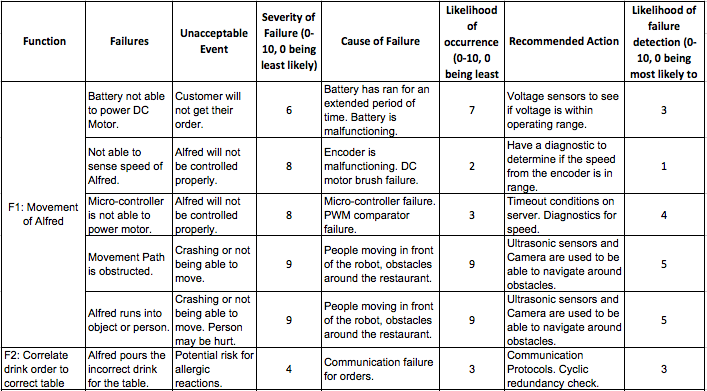
\includegraphics [scale = 0.7] {figures/FMEA_1.png}
	\caption{FMEA Table Part 1}
\end{figure}

\begin{figure} [H]
	\centering
	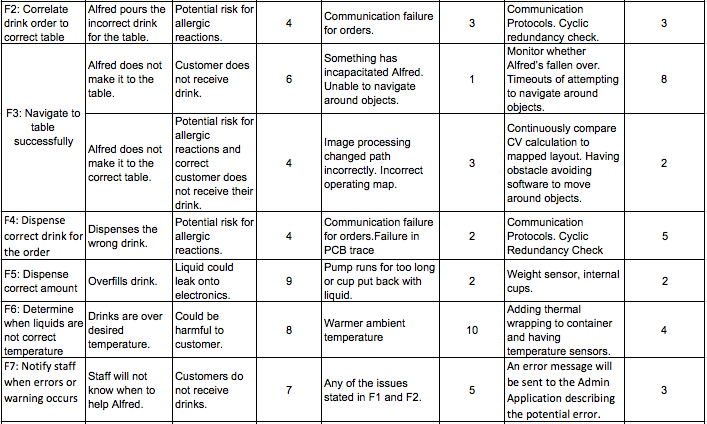
\includegraphics [scale = 0.7] {figures/FMEA_2.png}
	\caption{FMEA Table Part 2}
\end{figure}

\begin{figure} [H]
	\centering
	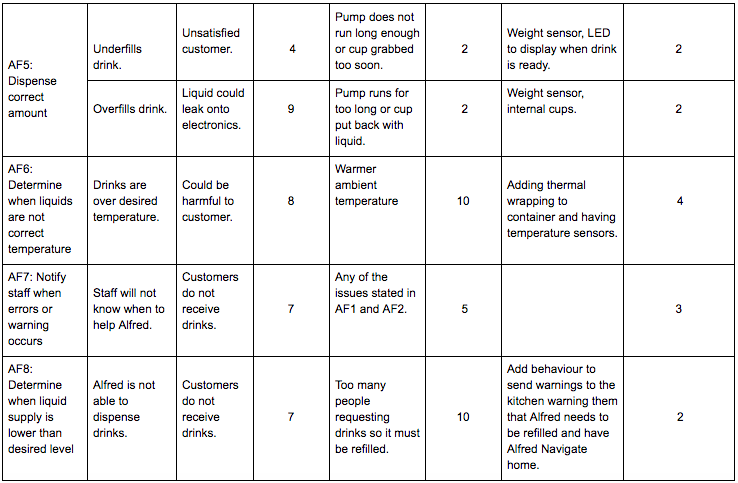
\includegraphics [scale = 0.7] {figures/FMEA_3.png}
	\caption{FMEA Table Part 3}
\end{figure}

\begin{figure} [H]
	\centering
	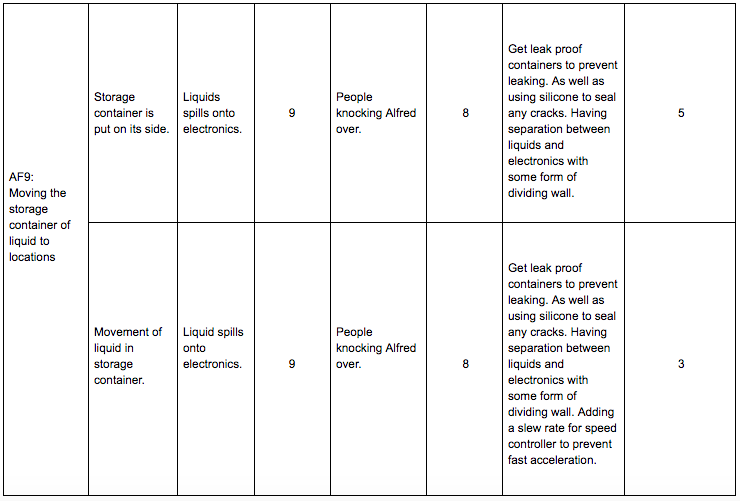
\includegraphics [scale = 0.7] {figures/FMEA_4.png}
	\caption{FMEA Table Part 4}
\end{figure}

\end{document}
